13. $y=\cfrac{2x^2-5x+2}{x-2}\cdot(x+1)=\cfrac{(2x-1)(x-2)}{x-2}\cdot(x+1)=2x^2+x-1,\ x\neq2.$ Построим параболу по трём точкам $(-1;0),\ \left(\cfrac{1}{2};0\right),\ \left(-\cfrac{1}{4};-\cfrac{9}{8}\right).$
$$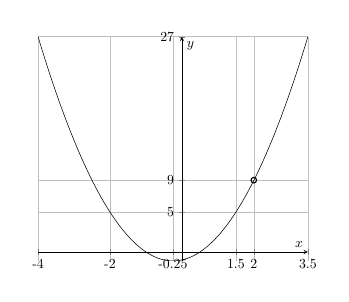
\begin{tikzpicture}[scale=0.5]
\begin{axis}[
    axis lines = middle,
    grid=major,
    legend pos={south west},
    xlabel = {$x$},
    ylabel = {$y$},
    %ymin=-80,
    %ymax=250,
    xtick={-4, -2, -0.25, 1.5,2, 3.5},
    xticklabels={-4, -2, -0.25, 1.5,2, 3.5},
    ytick={27,5,9},
    yticklabels={27,5,9}             ]
	\addplot[domain=-4:3.5, samples=100, color=black] {(2*x-1)*(x+1)};
%\addplot[domain=-3.1:2.5, samples=100, color=red] {70*abs(1-2*abs(abs(x)-2))-10*x^2+10*x-70};
	%\addlegendentry{$\text{Рис. 1}$};
\end{axis}
\draw (5.48,2.05) circle (2pt);
\end{tikzpicture}$$
